\documentclass{article}
\tracinglostchars=3 % Make it an error for letters to be missing.
\usepackage{enumitem}
\usepackage{babel}
\usepackage{unicode-math}
\usepackage{geometry}
\usepackage{tikz}
\usepackage{MnSymbol}
\usetikzlibrary{calc}
\usepackage{pgfplots}
\usepackage{multicol}
\usepackage{tcolorbox}
\usepackage{fancyhdr}
\usepackage{background}
\usepackage{array, makecell}
\pgfplotsset{compat=1.18}

\tikzstyle{process} = [rectangle, minimum width=3cm, minimum height=1cm, text centered, draw=black, fill=orange!30]
\tikzstyle{arrow} = [thick,->,>=stealth]

\geometry{left=1in, right=1in, top=1in, bottom=1in}
\pagestyle{fancy}

\babelprovide[import, onchar=fonts ids]{english}
\babelprovide[import, main, onchar=fonts ids]{thai}

\defaultfontfeatures{Scale=MatchLowercase, Ligatures=TeX}
\setmainfont{NewCM10-Regular.otf}
\babelfont{rm}
          [Scale=1.2]{NewCM10-Regular}
\babelfont[thai]{rm}
          [Weight=Regular, Scale=1.5]{TH Sarabun Chula}
% \setmathfont[Scale=1.2]{NewCMMath-Regular.otf}

% Define a command for Laplace transform with properly sized brackets
\newcommand{\laplace}[1]{\mathcal{L}\left\{#1\right\}}
% Optional: Define inverse Laplace transform command with properly sized brackets
\newcommand{\ilaplace}[1]{\mathcal{L}^{-1}\left\{#1\right\}}

\newcommand\encircle[1]{%
  \tikz[baseline=(X.base)] 
    \node (X) [draw, shape=circle, inner sep=0, fill=black, text=white] {\strut #1};%
}

\backgroundsetup{contents=
\includegraphics{kmutt-logo.png}, scale=0.7, opacity=0.03, angle=0}

\begin{document}
\fancyhead[L]{\textbf{คณิตศาสตร์วิศวกรรม} (Engineering Mathematics)}
\section{Introduction}
การแปลงลาปลาซ (Laplace Transform) เป็นเครื่องมือทางคณิตศาสตร์ที่ใช้ในการวิเคราะห์ระบบเชิงเส้นและการแก้สมการเชิงอนุพันธ์ (Differential Equation) โดยการแปลงฟังก์ชันตัวแปรจริง (ส่วนมากเป็นฟังก์ชันเวลา) $f(t)$ ให้เป็นฟังก์ชันตัวแปรเชิงซ้อน $s$ 
\begin{center}
    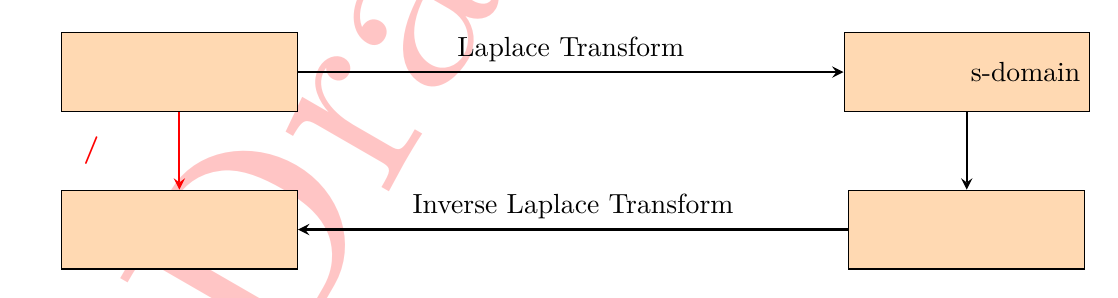
\begin{tikzpicture}
        \node (pro1) [process] {สมการเชิงอนุพันธ์เชิงเส้น};
        \node (pro2) [process, right of=pro1, node distance=10cm] {สมการพีชคณิตบน s-domain};
        \node (pro3) [process, below of=pro2, node distance=2cm] {ผลเฉลยของสมการพีชคณิต};
        \node (pro4) [process, left of=pro3, node distance=10cm] {ผลเฉลยของสมการเชิงอนุพันธ์};

            % Add arrows connecting the nodes
        \draw [arrow] (pro1) -- node[above, align=center] {Laplace Transform} (pro2);
        \draw [arrow] (pro2) -- (pro3);
        \draw [arrow] (pro3) -- node[above] {Inverse Laplace Transform} (pro4);
        \draw [arrow, color=red] (pro1) -- node[left, color=red] {\textbf{แก้ยาก/แก้ไม่ได้}} (pro4);
    \end{tikzpicture}
\end{center}
\vspace{0.1cm}
\begin{tcolorbox}[colback=gray!10, colframe=black!80]
    \textbf{บทนิยามการแปลงลาปลาซ}
    \begin{equation*}
        \laplace{f(t)} = F(s) = \int_0^\infty e^{-st} f(t) \; dt = \lim_{T \to \infty} \int_0^T e^{-st} f(t) \; dt
    \end{equation*}
\end{tcolorbox}
จะเห็นได้ว่าการแปลงลาปลาซนิยามโดยใช้การอินทิกรัลไม่ตรงแบบ (Improper Integral)
\section{Improper Integral}
อินทิกรัลไม่ตรงแบบ (Improper Integral) เป็นอินทิกรัลที่ทำบนช่วงที่ไม่มีขอบเขต หรือกับฟังก์ชันที่ไม่มีขอบเขต เมื่อ $f(x)$ เป็นฟังก์ชันต่อเนื่องบนช่วง $[a,b]$ 
\begin{enumerate}[label=\arabic*.]
    \item อินทิกรัลที่ไม่จำกัดขอบเขต (Infinite Interval)
        \begin{equation*}
            \lim_{b \to \infty} \int_a^b f(x) \; dx \quad \text{หรือ} \quad \lim_{a \to -\infty} \int_a^b f(x) \; dx \quad \text{หรือ} \quad \int_{-\infty}^\infty f(x) \; dx
        \end{equation*}
        \begin{multicols}{2}
            \begin{enumerate}[label=\alph*.]
                \item ลู่เข้า (Converge) เมื่อลิมิตหาค่าได้และค่าจำกัด
                \item ลู่ออก (Diverge) เมื่อไม่เข้าข้อ a.
            \end{enumerate}
        \end{multicols}
        \encircle{Q} จงหาว่าอินทิกรัลต่อไปนี้ลู่เข้าหรือลู่ออก ถ้าลู่เข้าจงหาค่าของอินทิกรัล \\
        \begin{multicols}{3}
            \noindent
            \begin{align*}
                \int_0^\infty e^{-x} \; dx
                &= \lim_{b \to \infty} \int_0^b e^{-x} \; dx \\
                &= \lim_{b \to \infty} \left[ -e^{-x} \right]_0^b \\
                &= \lim_{b \to \infty} \left( -e^{-b} + 1 \right) \\
                &= 1 \\
                \therefore \text{ อินทิกรัลลู่เข้า} &\text{และมีค่าเท่ากับ 1}
            \end{align*}
            \begin{equation*}
                \int_0^\infty x^2 e^{-x} \; dx
            \end{equation*}
            \columnbreak
            \begin{equation*}
                \int_{-\infty}^0 \frac{e^x}{3-2e^x} \; dx
            \end{equation*}
        \end{multicols}
        \newpage
    \item อินทิกรัลที่มีฟังก์ชันที่ไม่ต่อเนื่อง (Discontinuous Integrand)
        \begin{equation*}
            \int_a^b f(x) \; dx \quad \text{โดย} \quad f(x) \to \infty \text{ ที่ } x = c
        \end{equation*}
        \begin{multicols}{2}
            \begin{enumerate}[label=\alph*.]
                \item ลู่เข้า (Converge) เมื่อลิมิตหาค่าได้และค่าจำกัด
                \item ลู่ออก (Diverge) เมื่อไม่เข้าข้อ a.
            \end{enumerate}
        \end{multicols}
        \encircle{Q} จงหาว่าอินทิกรัลต่อไปนี้ลู่เข้าหรือลู่ออก ถ้าลู่เข้าจงหาค่าของอินทิกรัล \\
        \begin{multicols}{3}
            \noindent
            \begin{align*}
                &\int_1^2 \frac{x}{\sqrt{x^2-1}} \; dx \\
                &= \lim_{b \to 1^+} \int_b^2 \frac{x}{\sqrt{x^2-1}} \; dx \\
                &= \lim_{b \to 1^+} \left[ \sqrt{x^2-1} \right]_b^2 \\
                &= \sqrt{2^2-1} - \lim_{b \to 1^+} \sqrt{b^2-1} \\
                &= \sqrt{3} - 0 \\
                &= \sqrt{3} \\
                \therefore &\text{ อินทิกรัลลู่เข้าและมีค่าเท่ากับ $\sqrt{3}$}
            \end{align*}
            \begin{equation*}
                \int_{0}^{1} x \ln(x) \; dx
            \end{equation*}
            \columnbreak
            \begin{equation*}
                \int_0^3 \frac{1}{x^2+2x-3} \; dx
            \end{equation*}
        \end{multicols}
    \item \textbf{พิเศษ:} แบบผสม (Mixed Type)
        \begin{equation*}
            \int_{-\infty}^\infty f(x) \; dx = \int_{-\infty}^a f(x) \; dx + \int_a^b f(x) \; dx + \int_b^\infty f(x) \; dx
        \end{equation*}
        โดยจะแบ่งช่วงอินทิกรัลออกเป็นช่วง ๆ ให้แต่ละช่วงมีจุดไม่ต่อเนื่องเพียงจุดเดียว \\
        \encircle{Q} จงหาว่าอินทิกรัลต่อไปนี้ลู่เข้าหรือลู่ออก ถ้าลู่เข้าจงหาค่าของอินทิกรัล
        
        \begin{multicols}{2}
            \noindent
            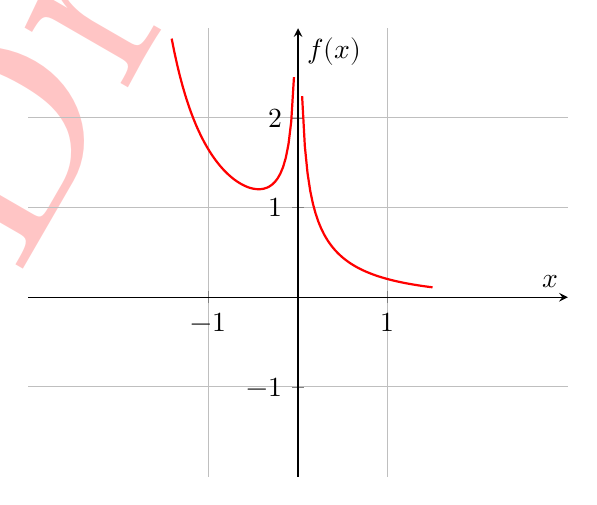
\begin{tikzpicture}
                \begin{axis}[
                    axis lines=middle,
                    xlabel={$x$},
                    ylabel={$f(x)$},
                    xtick={-1,0,1},
                    ytick={-1,0,1,2},
                    xmin=-1.5, xmax=1.5,
                    ymin=-2, ymax=3,
                    domain=-1.5:1.5,
                    restrict y to domain=-3:3,
                    samples=100,
                    grid=both,
                    axis equal
                ]
                    \addplot[red, thick] {
                        exp(-x/2) / (sqrt(abs(x)) * (x + 2))
                    };
                \end{axis}
            \end{tikzpicture}
            \columnbreak
            \begin{align*}
                \int_{-1}^\infty \frac{e^{-\frac{x}{2}}}{\sqrt{|x|}(x+2)} \; dx
            \end{align*}
        \end{multicols}
    \end{enumerate}
\pagebreak
\section{การแปลงลาปลาซ}
    จากความรู้เกี่ยวกับอินทิกรัลไม่ตรงแบบ เราสามารถใช้การแปลงลาปลาซในการวิเคราะห์ระบบเชิงเส้นได้ โดยการแปลงฟังก์ชัน $f(t)$ ให้เป็น $F(s)$ ซึ่งจะช่วยให้เราสามารถแก้สมการเชิงอนุพันธ์ได้ง่ายขึ้น \\
    \begin{tcolorbox}
    \textbf{ตัวช่วย: } Integration by Parts \\
    \begin{equation*}
        \int u \; dv = uv - \int v \; du
    \end{equation*}
    \textbf{ทบทวน: } บทนิยามการแปลงลาปลาซ \\
    \begin{equation*}
        \laplace{f(t)} = \lim_{T \to \infty} \int_0^T e^{-st} f(t) \; dt
    \end{equation*}
\end{tcolorbox}
\encircle{Q} จงหาผลการแปลงลาปลาซของฟังก์ชันต่อไปนี้\underline{โดยใช้บทนิยามการแปลงลาปลาซ}
\begin{multicols}{3}
    \noindent
    \begin{align*}
        f(t) &= 1 \\
        \laplace{f(t)} &= \int_0^\infty e^{-st} \cdot 1 \; dt \\
        &= \lim_{T \to \infty} \int_0^T e^{-st} \; dt \\
        &= \lim_{T \to \infty} \left[ -\frac{1}{s} e^{-st} \right]_0^T \\
        &= \lim_{T \to \infty} \left( -\frac{1}{s} e^{-sT} + \frac{1}{s} \right) \\
        &= \frac{1}{s} \quad \text{(เมื่อ $s > 0$)}
    \end{align*}
    \columnbreak
    \begin{align*}
        f(t) &= e^{-at} \\
    \end{align*}
    \columnbreak
    \begin{align*}
        f(t) &= t^2 \\
        % \laplace{f(t)} &= \int_0^\infty e^{-st} t^2 \; dt \\
        % &= \lim_{T \to \infty} \int_0^T e^{-st} t^2 \; dt \\
        % &= \lim_{T \to \infty} \left[ -\frac{1}{s} e^{-st} t^2 \right]_0^T + \frac{2}{s} \lim_{T \to \infty} \int_0^T e^{-st} t \; dt \\
        % &= \lim_{T \to \infty} \left( -\frac{1}{s} e^{-sT} T^2 + \frac{2}{s} \cdot \frac{1}{s^2} \right) \\
        % &= 0 + \frac{2}{s^3} \\
        % &= \frac{2}{s^3} \quad \text{(เมื่อ $s > 0$)}
    \end{align*}
\end{multicols}
\begin{multicols}{3}
    \noindent
    \begin{align*}
        f(t) = \sin(t)e^{-t}
    \end{align*}
\end{multicols}
\pagebreak
\subsection{สมบัติของการแปลงลาปลาซ}
\begin{tcolorbox}
    \noindent
    \begin{enumerate}[label=\arabic*.]
        \item \textbf{สมบัติเชิงเส้น (Linearity)}
        \begin{equation*}
            \laplace{af(t) + bg(t)} = a \laplace{f(t)} + b \laplace{g(t)}
        \end{equation*}
        โดยที่ $a$ และ $b$ เป็นค่าคงที่ 
        \item \textbf{การสเกล (Scaling)}
        \begin{equation*}
            \laplace{f(at)} = \frac{1}{a} F\left(\frac{s}{a}\right)
        \end{equation*}
        โดยที่ $a > 0$ และ $F(s) = \laplace{f(t)}$
        \item \textbf{การเลื่อนเวลา (Time Shifting)}
        \begin{equation*}
            \laplace{f(t - a) u(t - a)} = e^{-as} F(s)
        \end{equation*}
        โดยที่ $u(t - a)$ เป็นฟังก์ชันขั้นบันได (Unit Step Function) และ $a \geq 0$
        \item \textbf{การเลื่อนความถี่ (Frequency Shifting)}
        \begin{equation*}
            \laplace{e^{at} f(t)} = F(s - a)
        \end{equation*}
        โดยที่ $a$ เป็นค่าคงที่
        \item \textbf{การอนุพันธ์ (Differentiation)}
        \begin{equation*}
            \laplace{f'(t)} = s F(s) - f(0)
        \end{equation*}
        \begin{equation*}
            \laplace{f^{(n)}(t)} = s^n F(s) - s^{n-1} f(0) - s^{n-2} f'(0) - \ldots - f^{(n-1)}(0)
        \end{equation*}
        \item \textbf{การอนุพันธ์ในโดเมนความถี่ (Differentiation in Frequency Domain)}
        \begin{equation*}
            \laplace{t^n f(t)} = (-1)^n \frac{d^n}{ds^n} F(s)
        \end{equation*}
        \item \textbf{การอินทิกรัล (Integration)}
        \begin{equation*}
            \laplace{\int_0^t f(\tau) \; d\tau} = \frac{F(s)}{s}
        \end{equation*}
        \item \textbf{การอินทิกรัลในโดเมนความถี่ (Integration in Frequency Domain)}
        \begin{equation*}
            \laplace{\frac{f(t)}{t}} = \int_s^\infty F(u) \; du
        \end{equation*}
    \end{enumerate}
    \textbf{หมายเหตุ:} สมบัติของการแปลงลาปลาซเพิ่มเติมอยู่ในเอกสารประกอบการเรียนการสอน
\end{tcolorbox}
\pagebreak
\encircle{Q} จงหาผลการแปลงลาปลาซของฟังก์ชันต่อไปนี้โดยใช้สมบัติของการแปลงลาปลาซ
\begin{multicols}{2}
    \noindent
    \begin{align*}
        f(t) &= 4 - 3t + 2e^{-2t} \\
        % \laplace{f(t)} &= 4\laplace{1} - 3\laplace{t} + 2\laplace{e^{-2t}} \\
        % &= 4 \cdot \frac{1}{s} - 3 \cdot \frac{1}{s^2} + 2 \cdot \frac{1}{s+2} \\
        % &= \frac{4}{s} - \frac{3}{s^2} + \frac{2}{s+2}
    \end{align*}
    \columnbreak
    \begin{align*}
        f(t) &= t^2e^{3t} \\
        % \laplace{f(t)} &= \laplace{t^2e^{3t}} \\
        % &= \frac{d^2}{ds^2}\left[\laplace{e^{3t}}\right] \\
        % &= \frac{d^2}{ds^2}\left[\frac{1}{s-3}\right] \\
        % &= \frac{d}{ds}\left[\frac{1}{(s-3)^2}\right] \\
        % &= \frac{2}{(s-3)^3}
    \end{align*}
\end{multicols}
\vspace{3cm}

\begin{multicols}{2}
    \noindent
    \begin{align*}
        f(t) &= t\cos(2t) \\
        % \laplace{f(t)} &= \laplace{t\cos(2t)} \\
        % &= -\frac{d}{ds}\laplace{\cos(2t)} \\
        % &= -\frac{d}{ds}\left[\frac{s}{s^2+4}\right] \\
        % &= -\frac{(s^2+4) - s \cdot 2s}{(s^2+4)^2} \\
        % &= \frac{s^2-4}{(s^2+4)^2}
    \end{align*}
    \columnbreak
    \begin{align*}
        f(t) &= (t-3)^2u(t-3) \\
        % \laplace{f(t)} &= \laplace{(t-3)^2u(t-3)} \\
        % &= e^{-3s}\laplace{t^2} \quad \text{(เมื่อ $t-3=\tau$)} \\
        % &= e^{-3s} \cdot \frac{2}{s^3} \\
        % &= \frac{2e^{-3s}}{s^3}
    \end{align*}
\end{multicols}
\vspace{3cm}

\begin{multicols}{2}
    \noindent
    \begin{align*}
        f(t) &= \frac{4t+3}{t^2-5t+6} \\
    \end{align*}
    \columnbreak
    \begin{align*}
        f(t) &= \frac{d^2}{dt^2}(t^2\sin(t)) \\
    \end{align*}
\end{multicols}
\pagebreak
\begin{multicols}{2}
    \noindent
    \begin{align*}
        f(t) &= \int_0^t \sin{t} \cos{t} \; dt \\
    \end{align*}
    \begin{equation*}
    y(t) =
        \begin{cases}
            y'' - 2y' + 5y = 0 \\
            y(0) = 0, \quad y'(0) = 1
        \end{cases}
    \end{equation*}
\end{multicols}
\vspace{5cm}
\section{การแปลงลาปลาซผกผัน}
การแปลงลาปลาซผกผัน (Inverse Laplace Transform) เป็นกระบวนการที่ใช้ในการแปลงฟังก์ชัน $F(s)$ กลับไปเป็นฟังก์ชัน $f(t)$ โดยใช้สูตรการแปลงลาปลาซผกผัน \\
\encircle{Q} จงหาผลการแปลงลาปลาซผกผันของผลการแปลงลาปลาซต่อไปนี้
\begin{multicols}{2}
    \noindent
    \begin{align*}
        F(s) &= \frac{1}{s(s^2 + 4)} \\
    \end{align*}
    \columnbreak
    \begin{align*}
        F(s) &= \frac{6s - 5}{s^2 + 7} \\
    \end{align*}
\end{multicols}
\vspace{3cm}
\begin{multicols}{2}
    \noindent
    \begin{align*}
        F(s) &= \frac{s - 1}{s^2 - 2s + 5} \\
    \end{align*}
    \columnbreak
    \begin{align*}
        F(s) &= \frac{-2s}{(s^2 + 4)^2} \\
    \end{align*}
\end{multicols}
\pagebreak
\section{การแปลงฟูเรียร์}
การแปลงฟูเรียร์ (Fourier Transform) เป็นเครื่องมือทางคณิตศาสตร์ที่ใช้ในการวิเคราะห์สัญญาณและระบบ โดยการแปลงฟังก์ชัน $f(t)$ ให้เป็นฟังก์ชัน $F(\omega)$ ซึ่งเป็นฟังก์ชันของความถี่ $\omega$ \\
\begin{tcolorbox}
    \textbf{บทนิยามการแปลงฟูเรียร์} \\
    บทนิยามการแปลงฟูเรียร์นั้นมีหลายแบบ โดยที่นิยมใช้ในการวิเคราะห์สัญญาณได้นิยามไว้ดังนี้
    \begin{equation*}
        F(\omega) = \int_{-\infty}^\infty f(t) e^{-i\omega t} \; dt
    \end{equation*}
    \\
    \textbf{บทนิยามการแปลงฟูเรียร์ผกผัน}
    \begin{equation*}
        f(t) = \frac{1}{2\pi} \int_{-\infty}^\infty F(\omega) e^{i\omega t} \; d\omega
    \end{equation*}
    โดยที่ $i$ เป็นหน่วยจินตภาพ (Imaginary Unit) และ $\omega$ เป็นความถี่เชิงมุม (Angular Frequency, 2πf) \\
\end{tcolorbox}
\encircle{Q} จงหาผลการแปลงฟูเรียร์ของฟังก์ชันต่อไปนี้ โดยใช้บทนิยามการแปลงฟูเรียร์
\begin{multicols}{2}
    \noindent
    \begin{align*}
        f(t) &= e^{-at} \\
    \end{align*}
    \columnbreak
    \begin{align*}
        f(t) = 
        \begin{cases}
            \cos(3t) & \text{เมื่อ } t \geq 0 \\
            0 & \text{เมื่อ } t < 0
        \end{cases}
    \end{align*}
\end{multicols}
\vspace{5cm}
\begin{center}
    \renewcommand{\arraystretch}{2}
    \begin{tabular}{ll}
        \textbf{คุณสมบัติ} & \textbf{การแปลงฟูเรียร์} \\
        \hline
        \textbf{เชิงเส้น (Linearity)} & $F(a f(t) + b g(t)) = a F(f(t)) + b F(g(t))$ \\
        \textbf{การเลื่อนเวลา (Time Shifting)} & $F(f(t - a)) = e^{-i\omega a} F(f(t))$ \\
        \textbf{การสเกล (Scaling)} & $F(f(at)) = \frac{1}{|a|} F\left(\frac{\omega}{a}\right)$ \\
        \textbf{อนุพันธ์ (Differentiation)} & $F(f^{(n)}(t)) = (i\omega)^n F(f(t))$ \\
    \end{tabular}\\
\end{center}
\pagebreak
\encircle{Q} จงหาผลการแปลงฟูเรียร์ผกผันของผลการแปลงฟูเรียร์ต่อไปนี้
\begin{multicols}{2}
    \noindent
    \begin{align*}
        F(\omega) &= 20\frac{\sin(5\omega)}{5\omega} \\
    \end{align*}
    \columnbreak
    \begin{align*}
        F(\omega) &= \frac{e^{i\omega}}{1 + i\omega} \\
    \end{align*}
\end{multicols}
\pagebreak
\section{Formulas}
\renewcommand{\arraystretch}{2.5}
    \begin{center}
        \begin{tabular}{|p{0.45\textwidth}|p{0.45\textwidth}|}
            \hline
            \multicolumn{1}{|c|}{\textbf{Derivatives}} & \multicolumn{1}{c|}{\textbf{Integrals}} \\
            \hline
            $\displaystyle\frac{d}{dx}(a) = 0$ & $\displaystyle\int a \,dx = ax + C$ \\
            $\displaystyle\frac{d}{dx}(x^n) = nx^{n-1}$ & $\displaystyle\int x^n \,dx = \frac{x^{n+1}}{n+1} + C, n \neq -1$ \\
            $\displaystyle\frac{d}{dx}(e^x) = e^x$ & $\displaystyle\int e^x \,dx = e^x + C$ \\
            $\displaystyle\frac{d}{dx}(a^x) = a^x \ln(a)$ & $\displaystyle\int a^x \,dx = \frac{a^x}{\ln(a)} + C$ \\
            $\displaystyle\frac{d}{dx}(\ln|x|) = \frac{1}{x}$ & $\displaystyle\int \frac{1}{x} \,dx = \ln|x| + C$ \\
            $\displaystyle\frac{d}{dx}(\log_a|x|) = \frac{1}{x\ln(a)}$ & $\displaystyle\int x^{-1} \,dx = \ln|x| + C$ \\
            $\displaystyle\frac{d}{dx}(\sin x) = \cos x$ & $\displaystyle\int \sin x \,dx = -\cos x + C$ \\
            $\displaystyle\frac{d}{dx}(\cos x) = -\sin x$ & $\displaystyle\int \cos x \,dx = \sin x + C$ \\
            $\displaystyle\frac{d}{dx}(\tan x) = \sec^2 x$ & $\displaystyle\int \tan x \,dx = -\ln|\cos x| + C$ \\
            $\displaystyle\frac{d}{dx}(\cot x) = -\csc^2 x$ & $\displaystyle\int \cot x \,dx = \ln|\sin x| + C$ \\
            $\displaystyle\frac{d}{dx}(\sec x) = \sec x \tan x$ & $\displaystyle\int \sec x \,dx = \ln|\sec x + \tan x| + C$ \\
            $\displaystyle\frac{d}{dx}(\csc x) = -\csc x \cot x$ & $\displaystyle\int \csc x \,dx = \ln|\csc x - \cot x| + C$ \\
            $\displaystyle\frac{d}{dx}(\sinh x) = \cosh x$ & $\displaystyle\int \sinh x \,dx = \cosh x + C$ \\
            $\displaystyle\frac{d}{dx}(\cosh x) = \sinh x$ & $\displaystyle\int \cosh x \,dx = \sinh x + C$ \\
            $\displaystyle\frac{d}{dx}(f \pm g) = \frac{df}{dx} \pm \frac{dg}{dx}$ & $\displaystyle\int (f \pm g) \,dx = \int f \,dx \pm \int g \,dx$ \\
            $\displaystyle\frac{d}{dx}(fg) = f\frac{dg}{dx} + g\frac{df}{dx}$ & $\displaystyle\int f g' \,dx = fg - \int f' g \,dx$ \\
            $\displaystyle\frac{d}{dx}(\frac{f}{g}) = \frac{g\frac{df}{dx} - f\frac{dg}{dx}}{g^2}$ & $\displaystyle\int \frac{f'(x)}{f(x)} \,dx = \ln|f(x)| + C$ \\
            $\displaystyle\frac{d}{dx}(f(g(x))) = f'(g(x))g'(x)$ & $\displaystyle\int f'(g(x))g'(x) \,dx = f(g(x)) + C$ \\
            \hline
        \end{tabular}
    \end{center}
\pagebreak
    \begin{center}
    \renewcommand{\arraystretch}{3.5}
        \begin{tabular}{|p{0.35\textwidth}|p{0.65\textwidth}|}
            \hline
            \multicolumn{2}{|c|}{\textbf{Laplace Transform Formulas} $\displaystyle\newline{\laplace{f(t)} = F(s) = \int_0^\infty e^{-st} f(t) \; dt}$} \\
            \hline
            $\displaystyle\laplace{k} = \frac{k}{s},\quad k \text{ constant}$ & $\displaystyle\laplace{\sin at} = \frac{a}{s^2 + a^2} $ \\
            $\displaystyle\laplace{t^n} = \frac{n!}{s^{n+1}},\quad n=1,2,\dots$ & $\displaystyle\laplace{\cos at} = \frac{s}{s^2 + a^2} $ \\
            $\displaystyle\laplace{t^a} = \frac{\Gamma(a+1)}{s^{a+1}},\quad a > -1 $ & $\displaystyle\laplace{\sinh at} = \frac{a}{s^2 - a^2} $ \\
            $\displaystyle\laplace{e^{at}} = \frac{1}{s - a} $ & $\displaystyle\laplace{\cosh at} = \frac{s}{s^2 - a^2} $ \\
            $\displaystyle\laplace{t \sin at} = \frac{2as}{(s^2 + a^2)^2} $ & $\displaystyle\laplace{t \cos at} = \frac{s^2 - a^2}{(s^2 + a^2)^2} $ \\
            $\displaystyle\laplace{\frac{\sin at}{t}} = \tan^{-1}\left(\frac{a}{s}\right)$ & $\displaystyle\laplace{a_1 f_1(t) + a_2 f_2(t)} = a_1 \laplace{f_1(t)} + a_2 \laplace{f_2(t)}$ \\
            $\displaystyle\laplace{e^{at} f(t)} = F(s - a)$ & $\displaystyle\laplace{t^n f(t)} = (-1)^n \frac{d^n}{ds^n}F(s)$ \\
            $\displaystyle\laplace{\frac{f(t)}{t}} = \int_s^\infty F(u)\,du$ & $\displaystyle\laplace{f^{(n)}(t)} = s^nF(s) - s^{n-1}f(0) - \cdots - f^{(n-1)}(0)$ \\
            $\displaystyle\laplace{\int_0^t f(u)\,du} = \frac{F(s)}{s}$ & $\displaystyle\laplace{f(t) * g(t)} = F(s)G(s) \newline{\text{where} \; (f * g)(t) = \int_0^t f(\tau) g(t - \tau)\,d\tau}$ \\
            $\displaystyle\laplace{u(t - a)} = \frac{e^{-as}}{s}$ & $\displaystyle\laplace{f(t)u(t - a)} = e^{-as} \laplace{f(t + a)} \newline{\text{where} \; u(t - a) \text{ is the unit step function}}$ \\
            & $\displaystyle\laplace{f(t)} = \frac{1}{1 - e^{-Ts}} \int_0^T e^{-st} f(t)\,dt \quad \text{if } f(t + T) = f(t)$ \\         
            \hline
        \end{tabular}
    \end{center}
\end{document}